\documentclass[UTF8,a4paper,12pt, onecolumn]{ctexart}
\usepackage[left=2.50cm, right=2.50cm, top=2.50cm, bottom=2.50cm]{geometry}

% -- text font --
% compile using Xelatex

%\setmainfont{Microsoft YaHei}  % 微软雅黑
%\setmainfont{YouYuan}  % 幼圆    
%\setmainfont{NSimSun}  % 新宋体
%\setmainfont{KaiTi}    % 楷体
\setmainfont{Songti SC}   % 宋体
%\setmainfont{SimHei}   % 黑体

\usepackage{times}
%\usepackage{mathpazo}
%\usepackage{fourier}
%\usepackage{charter}
%\usepackage{helvet}

\usepackage{amsmath, amsfonts, amssymb} % math equations, symbols
%\usepackage[english]{babel}
\usepackage{color}      % color content
\usepackage{graphicx}   % import figures
\usepackage{url}        % hyperlinks
\usepackage{bm}         % bold type for equations
\usepackage{multirow}
\usepackage{booktabs}
\usepackage{epstopdf}
\usepackage{epsfig}
\usepackage{algorithm}
\usepackage{algorithmic}
\renewcommand{\algorithmicrequire}{ \textbf{Input:}}     % use Input in the format of Algorithm  
\renewcommand{\algorithmicensure}{ \textbf{Initialize:}} % use Initialize in the format of Algorithm  
\renewcommand{\algorithmicreturn}{ \textbf{Output:}}     % use Output in the format of Algorithm  

\usepackage{fancyhdr}   % 设置页眉、页脚
%\pagestyle{fancy}
\lhead{}
\chead{}
%\rhead{\includegraphics[width=1.2cm]{}}
\lfoot{}
\cfoot{}
\rfoot{}

\usepackage{gbt7714}
%\renewcommand{\refname}{参考文献}   % 将References改为参考文献

%\usepackage{draftwatermark}         % 所有页加水印
%\usepackage[firstpage]{draftwatermark} % 只有第一页加水印
%\SetWatermarkText{Water-Mark}           % 设置水印内容
%\SetWatermarkText{\includegraphics{}}         % 设置水印logo
%\SetWatermarkLightness{0.9}             % 设置水印透明度 0-1
%\SetWatermarkScale{1}                   % 设置水印大小 0-1    

\usepackage{hyperref}   % bookmarks
\hypersetup{colorlinks, bookmarks, unicode} % unicode
\usepackage{pdfpages}

\title{人工智能疾病诊断平台\\AI.sdu.edu.cn}
\author{薛付忠~教授\thanks{山东大学健康医疗大数据研究院}}
\date{\today}


\begin{document}
    \maketitle
    \thispagestyle{fancy}
    
\tableofcontents

\section{项目背景}



\section{平台需求}

\subsection{用户角色}

平台主要包括三类用户:普通用户、医疗机构用户和平台管理员。普通用户,是指自行注册的个人用户;医疗机构用户,是指针对各医疗机构由平台管理员审核并分配的用户;平台管理员是平台内置的管理用户,可根据管理权限分级需要,设置多个管理员账号。

\subsection{功能需求}

\subsubsection{平台注册}

普通用户,可以通过手机APP、微信小程序或网页版平台自行注册,可以用手机号作为首选身份认证,用户名和密码作为次选身份认证。

医疗机构用户,由平台管理员审核分配,医疗机构可以申请注册医疗机构用户,并能平台管理员审核分配账号。医疗机构申请注册时,需提供机构相关证明用于资质审核,以及负责人手机号用于接收平台通知和密码找回等功能。

平台管理员账号,通过平台数据初始化或代码配置的方式内置在平台中。可根据安全级别,限制登录区域和记录操作行为。

\subsubsection{账户管理}

普通用户,可以管理维护个人的相关信息,如:更换手机号和相关隐私设置等。普通用户选填信息包括:姓名、性别、出生日期、身份证号、职业、家庭地址等。其中,家庭地址按省市县镇等行政区域级别选择输入,职业按固定列表选择输入,便于后期的数据统计。性别、出生日期增加保密选项,减少用户提供虚假信息带来的统计数据干扰。

医疗机构用户,可以维护所在机构的基本信息,如:机构介绍、等级、地址等,可以更换负责人手机号。

\subsubsection{病例管理}

医疗机构用户,可以在平台上建立机构的病例档案,跟踪各病例的诊断记录。病例档案可以按手机号或身份证号作为唯一标识。

普通用户,可根据手机号或身份证号匹配查看个人在医疗机构的病例档案。

\subsubsection{诊断功能}

诊断功能是平台提供的核心功能。目前,平台仅提供血液疾病的诊断功能,其它疾病诊断功能待诊断模型开发完成后陆续上线。

血液疾病诊断功能流程如下图所示。

\subsubsection{代码对照表管理}

针对平台管理员开放。

\begin{itemize}
  \item 行政区域代码表
  \item 职业代码表
  \item 疾病代码表
\end{itemize}

\subsubsection{其它衍生功能}

\begin{itemize}
  \item 数据统计(疾病、地区、年龄)
  \item 就医指导
  \item 诊断模型升级
\end{itemize}

\subsection{原型系统需求}

\begin{figure}
	\centering
	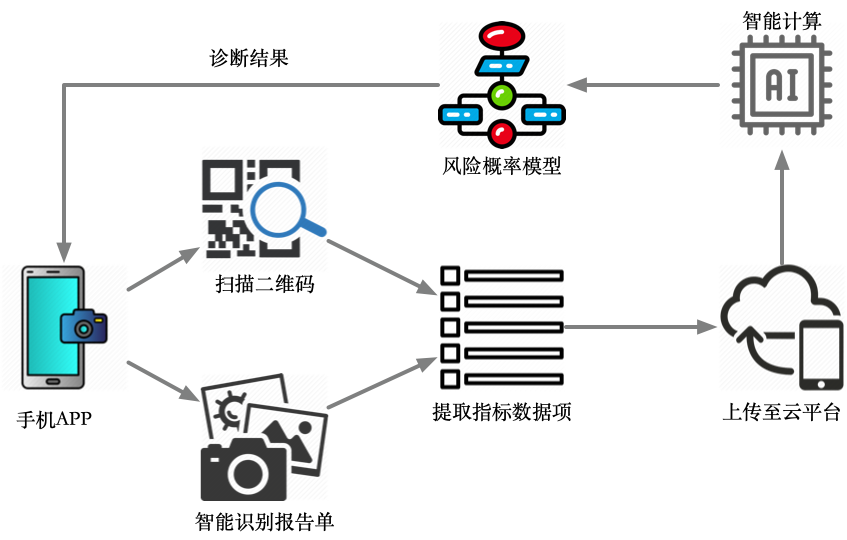
\includegraphics[width=\textwidth]{images/prototype.png}
	\caption{原型系统流程图}
\end{figure}

\section{构架设计}



\section{开发框架}



\section{系统部署}


%\bibliography{blood-references.bib}

\appendix

\end{document}